\begin{center}
\Huge
	Omdrejningslegemer og kurvelængder
\end{center}

\section*{Rumfang af omdrejningslegemer}
\stepcounter{section}

Hvis vi roterer grafen for en kontinuert funktion $f$ omkring $x$-aksen på et interval $[a,b]$, så vil dette danne hvad vi kalder for et \textit{omdrejningslegeme}. Vi kan se et eksempel på et omdrejningslegeme på Figur \ref{fig:omdrejning}.
\begin{figure}[H]
	\centering
	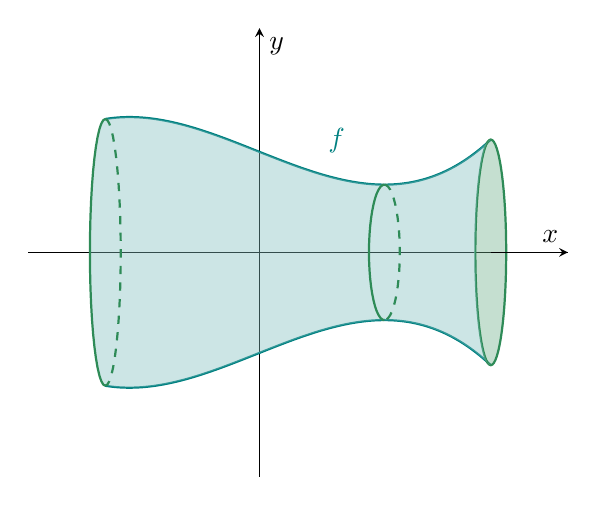
\begin{tikzpicture}
	\begin{axis}[
	axis lines = center, 
	xmin = -3, xmax = 4,
	ymin = -6, ymax = 6,
	ticks = none,
	xlabel = $x$, ylabel = $y$
	]
		\addplot[color = teal, thick, domain = -2:3, samples = 500] {0.1*x^(3) + 0.01*x^(2) - 0.82*x + 2.69};
		\addplot[color = teal, thick, domain = -2:3, samples = 500] {-(0.1*x^(3) + 0.01*x^(2) - 0.82*x + 2.69)};
		\filldraw[color = SeaGreen!70, opacity = 0.4] (axis cs: 3,0) ellipse (0.2 and {151/50});
		\draw[color = SeaGreen, thick] (axis cs: 3,0) ellipse (0.2 and {151/50});
		\draw[] (axis cs: 3,0) -- (axis cs: 4,0);
		\node[color = teal] at (axis cs: 1,3) {$f$};
		%Filling
		\fill[color = teal!50, opacity = 0.4] 
		plot[domain = -2:3, variable = \x] (axis cs: \x, {0.1*(\x)^3 + 0.01*(\x)^2 - 0.82*\x + 2.69}) --
		plot[domain = 90:270, variable = \t] (axis cs: {0.2*cos(\t) + 3} , {151/50 * sin(\t)}) -- 
		plot[domain = 3:-2, variable = \x] (axis cs: \x, {-(0.1*(\x)^3 + 0.01*(\x)^2 - 0.82*\x + 2.69)}) --
		plot[domain = 270:90, variable = \t] (axis cs: {0.2*cos(\t) - 2} , {3.57 * sin(\t)})	-- cycle;
		%Circles
		%Left circle
		\draw[color = SeaGreen, thick]
		plot[domain = 90:270, variable = \t] (axis cs: {0.2*cos(\t) - 2} , {3.57 * sin(\t)});
		\draw[color = SeaGreen, thick, dashed]
		plot[domain = 90:-90, variable = \t] (axis cs: {0.2*cos(\t) - 2} , {3.57 * sin(\t)});
		%Middle circle
		\draw[color = SeaGreen, thick]
		plot[domain = 90:270, variable = \t] (axis cs: {0.2*cos(\t) + 1.62} , {1.813 * sin(\t)});
		\draw[color = SeaGreen, thick, dashed]
		plot[domain = 90:-90, variable = \t] (axis cs: {0.2*cos(\t) + 1.62} , {1.813 * sin(\t)});
	\end{axis}
	\end{tikzpicture}
	\caption{Omdrejningslegeme for funktion $f$. }
	\label{fig:omdrejning}
\end{figure}

Følgende sætning giver os volumen af et omdrejningslegeme for en kontinuert funktion. 
\begin{setn}[Volumen af omdrejningslegeme]
	For en kontinuert funktion $f$ er volumen af omdrejningslegemet på intervallet $[a,b]$ givet ved
	\begin{align*}
		\pi \int_a^b(f(x))^2 dx.	
	\end{align*}	 
\end{setn}
\begin{proof}
	\begin{figure}[H]
	\centering
	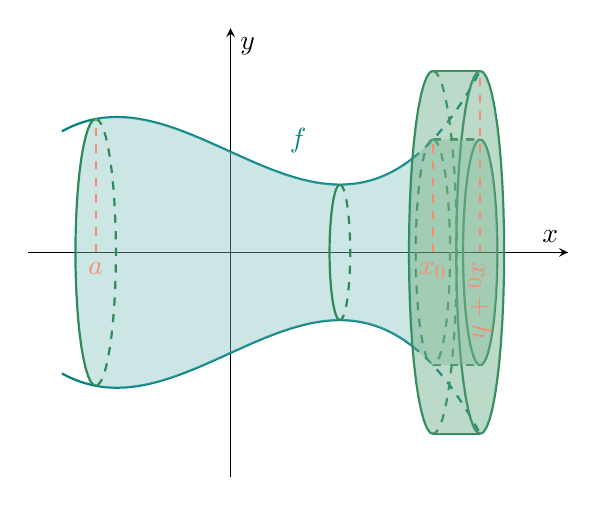
\begin{tikzpicture}
	\begin{axis}[
	axis lines = center, 
	xmin = -3, xmax = 5,
	ymin = -6, ymax = 6,
	ticks = none,
	xlabel = $x$, ylabel = $y$
	]
		\addplot[color = teal, thick, domain = -2.5:2.7, samples = 500] {0.1*x^(3) + 0.01*x^(2) - 0.82*x + 2.69};
		\addplot[color = teal, thick, domain = -2.5:2.7, samples = 500] {-(0.1*x^(3) + 0.01*x^(2) - 0.82*x + 2.69)};
		\addplot[color = teal, thick, domain = 2.7:3.7, samples = 200, dashed] {0.1*x^(3) + 0.01*x^(2) - 0.82*x + 2.69};
		\addplot[color = teal, thick, domain = 2.7:3.7, samples = 200, dashed] {-(0.1*x^(3) + 0.01*x^(2) - 0.82*x + 2.69)};
		\draw[] (axis cs: 3,0) -- (axis cs: 5,0);
		\node[color = teal] at (axis cs: 1,3) {$f$};
		%Filling
		\fill[color = teal!50, opacity = 0.4] 
		plot[domain = -2:3, variable = \x] (axis cs: \x, {0.1*(\x)^3 + 0.01*(\x)^2 - 0.82*\x + 2.69}) --
		plot[domain = 90:270, variable = \t] (axis cs: {0.254*cos(\t) + 3} , {151/50 * sin(\t)}) -- 
		plot[domain = 3:-2, variable = \x] (axis cs: \x, {-(0.1*(\x)^3 + 0.01*(\x)^2 - 0.82*\x + 2.69)}) --
		plot[domain = 270:90, variable = \t] (axis cs: {0.3*cos(\t) - 2} , {3.57 * sin(\t)})	-- cycle;
		%Circles
		%Left circle
		\draw[color = SeaGreen, thick]
		plot[domain = 90:270, variable = \t] (axis cs: {0.30*cos(\t) - 2} , {3.57 * sin(\t)});
		\draw[color = SeaGreen, thick, dashed]
		plot[domain = 90:-90, variable = \t] (axis cs: {0.30*cos(\t) - 2} , {3.57 * sin(\t)});
		%Middle left circle
		\draw[color = SeaGreen, thick]
		plot[domain = 90:270, variable = \t] (axis cs: {0.153*cos(\t) + 1.62} , {1.813 * sin(\t)});
		\draw[color = SeaGreen, thick, dashed]
		plot[domain = 90:-90, variable = \t] (axis cs: {0.153*cos(\t) + 1.62} , {1.813 * sin(\t)});
		%Middle right circle
		\draw[color = SeaGreen, thick, dashed]
		plot[domain = 90:270, variable = \t] (axis cs: {0.254*cos(\t) + 3} , {3.02 * sin(\t)});
		\draw[color = SeaGreen, thick, dashed]
		plot[domain = 90:-90, variable = \t] (axis cs: {0.254*cos(\t) + 3} , {3.02 * sin(\t)});
		\draw[color = SeaGreen, thick]
		plot[domain = 90:270, variable = \t] (axis cs: {0.355*cos(\t) + 3} , {4.858 * sin(\t)});
		\draw[color = SeaGreen, thick, dashed]
		plot[domain = 90:-90, variable = \t] (axis cs: {0.355*cos(\t) + 3} , {4.858 * sin(\t)});
		%Right circles
		\draw[color = SeaGreen, thick]
		plot[domain = 90:270, variable = \t] (axis cs: {0.355*cos(\t) + 3.7} , {4.858 * sin(\t)});
		\draw[color = SeaGreen, thick]
		plot[domain = 90:-90, variable = \t] (axis cs: {0.355*cos(\t) + 3.7} , {4.858 * sin(\t)});
		\draw[color = SeaGreen, thick]
		plot[domain = 90:270, variable = \t] (axis cs: {0.254*cos(\t) + 3.7} , {3.02 * sin(\t)});
		\draw[color = SeaGreen, thick]
		plot[domain = 90:-90, variable = \t] (axis cs: {0.254*cos(\t) + 3.7} , {3.02 * sin(\t)});
		%horisontal lines 
		\draw[color = SeaGreen, thick, dashed] (axis cs: 3,3.02) -- (axis cs: 3.7,3.02);
		\draw[color = SeaGreen, thick, dashed] (axis cs: 3,-3.02) -- (axis cs: 3.7,-3.02);
		\draw[color = SeaGreen, thick] (axis cs: 3,4.858) -- (axis cs: 3.7,4.858);
		\draw[color = SeaGreen, thick] (axis cs: 3,-4.858) -- (axis cs: 3.7,-4.858); 
		%Cylinder fill
		\fill[color = SeaGreen!50, opacity = 0.4]
		plot[domain = 90:-90, variable = \t] (axis cs: {0.254 * cos(\t) + 3.7} , {3.02 * sin(\t)}) --
		plot[domain = 270:90, variable = \t] (axis cs: {0.254 * cos(\t) + 3} , {3.02 * sin(\t)}) -- cycle;
		\fill[color = SeaGreen!80, opacity = 0.4]
		plot[domain = 90:-90, variable = \t] (axis cs: {0.355 * cos(\t) + 3.7} , {4.858 * sin(\t)}) --
		plot[domain = 270:90, variable = \t] (axis cs: {0.355 * cos(\t) + 3} , {4.858 * sin(\t)}) -- cycle;
		%Ticks and dashes
		\node[color = Melon, anchor = north] at (axis cs: -2,0) {$a$};
		\draw[color = Melon, thick, dashed] (axis cs: -2,0) -- (axis cs: -2, 3.57);
		\node[color = Melon, anchor = north] at (axis cs: 3,0) {$x_0$};
		\draw[color = Melon, thick, dashed] (axis cs: 3,0) -- (axis cs: 3, 3.02);
		\node[color = Melon, anchor = west, rotate = -90] at (axis cs: 3.7, 0) {$x_0 + h$};
		\draw[color = Melon, thick, dashed] (axis cs: 3.7 ,0) -- (axis cs: 3.7, 4.858);
	\end{axis}
	\end{tikzpicture}
	\caption{Approksimation af omdregningslegeme.}
	\label{fig:bevis}
	\end{figure}
	Til beviset tager vi udgangspunkt i Figur \ref{fig:bevis}. Vi starter med at antage, at der findes en
	 rumfangsfunktion 
	 \begin{align*}
	 	R_a(x),
	 \end{align*}
	 der giver os rumfanget af omdrejningslegemet fra $a$ til $x$. Vi antager desuden, at den betragtede funktion $f$ er 
	 voksende i omegnen af $x_0$ som det er tilfældet på Figur \ref{fig:bevis} samt at $h > 0$. 
	  Vi ønsker at betragte arealet fra $a$ til $x_0 + h$ 
	 som set på Figur \ref{fig:bevis}. Vi starter med at overveje rumfanget af de to cylindre på figuren. 
	 Den lille cylinder har en højde på $h$ og en radius på $f(x_0)$, så rumfanget af denne cylinder er 
	 $h \pi (f(x_0))^2$. 
	 Den store cylinder har en højde på $h$ og en radius på $f(x_0 + h)$, så rumfanget af denne cylinder er 
	 $h \pi (f(x_0 + h))^2$. Disse kan vi bruge til at approksimere rumfanget $R_a(x_0+h)$. Der må gælde følgende
	 ulighed	 for rumfanget.
	 \begin{align*}
	 	R_a(x_0 + h) \leq R_a(x_0) +  \pi h (f(x_0 + h))^2,
	\end{align*}	  
	altså at rumfanget er mindre end rumfanget hen til $x_0$ lagt sammen med den store cylinder. Tilsvarende har vi
	\begin{align*}
		R_a(x_0 + h) \geq R_a(x_0) +  \pi h (f(x_0))^2, 
	\end{align*}
	altså at rumfanget er større end rumfanget hen til $x_0$ lagt sammen med den lille cylinder. Vi kan samle disse til
	\begin{align*}
		R_a(x_0) + \pi h (f(x_0))^2 \leq R_a(x_0 + h) \leq R_a(x_0) + \pi h (f(x_0 + h))^2
	\end{align*}
	Vi trækker nu $R_a(x_0)$ fra samt dividerer med $h$. Dette giver
	\begin{align*}
		&R_a(x_0) + \pi h (f(x_0))^2 \leq R_a(x_0 + h) \leq R_a(x_0) + \pi h (f(x_0 + h))^2 \\
		\Leftrightarrow \ &\pi h (f(x_0))^2 \leq R_a(x_0 + h) - R_a(x_0) \leq \pi h (f(x_0 + h))^2 \\
		\Leftrightarrow \ &\pi(f(x_0))^2 \leq \frac{R_a(x_0 + h) - R_a(x_0)}{h} \leq \pi(f(x_0 + h))^2
	\end{align*}
	Vi lader nu $h \to 0$, da det midterste udtryk genkendes som en differenskvotient.
	\begin{align*}
		&\lim_{h \to 0}\pi(f(x_0))^2 \leq \lim_{h \to 0}\frac{R_a(x_0 + h) - R_a(x_0)}{h} \leq
		 \lim_{h \to 0}\pi(f(x_0 + h))^2 \\
		 \Leftrightarrow \ & \pi (f(x_0))^2 \leq R_a'(x_0) \leq \pi (f(x_0))^2 \\
		 \Leftrightarrow \ & \pi (f(x_0))^2 = R_a'(x_0).
	\end{align*}
	Vi udnytter her, at $f$ er kontinuert, så $\displaystyle \lim_{h\to 0} \pi (f(x_0 + h))^2 = \pi (f(x_0))^2$.
	Dette betyder derfor, at $R_a$ er en stamfunktion til $\pi (f(x_0))^2$. Vi får derfor
	\begin{align*}
		\int_a^b \pi (f(x))^2 dx = R_a(b) - R_a(a) = R_a(b),
	\end{align*}
	hvilket jo netop er rumfanget fra $a$ til $b$. 
\end{proof}

\begin{exa}
	En funktion $f$ er givet ved 
	\begin{align*}
		f(x) = \frac{1}{x},
	\end{align*}
	og grafen for funktionen samt omdrejningslegemet for $f$ på intervallet $[2,5]$ kan ses på Figur
	 \ref{fig:omdrejningexa}
	 \begin{figure}[H]
	\centering
	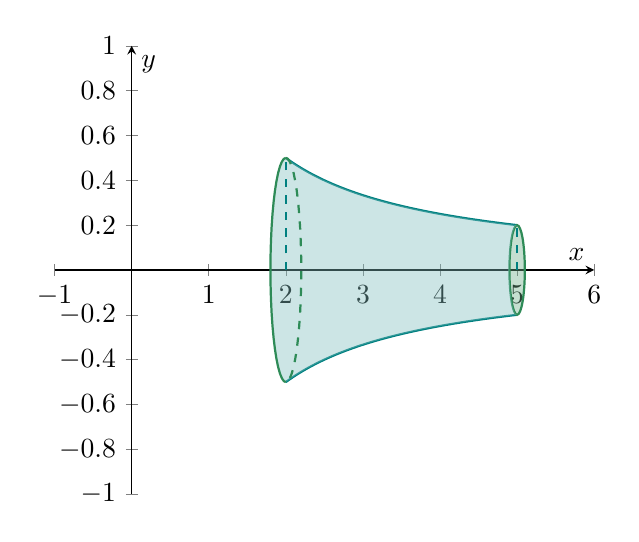
\begin{tikzpicture}
	\begin{axis}[
	axis lines = center, 
	xmin = -1, xmax = 6,
	ymin = -1, ymax = 1,
	xlabel = $x$, ylabel = $y$,
	xtick = {-2,-1,...,5,6}, ytick = {-1,-0.8,...,0.8,1},
	]
		\addplot[color = teal, thick, domain = 2:5, samples = 500] {1/x};
		\addplot[color = teal, thick, domain = 2:5, samples = 500] {-1/x};
		\filldraw[color = SeaGreen!70, opacity = 0.4] (axis cs: 5,0) ellipse (0.1 and {1/5});
		\draw[color = SeaGreen, thick] (axis cs: 5,0) ellipse (0.1 and {1/5});
		\node[color = teal] at (axis cs: 1,3) {$f$};
		%Filling
		\fill[color = teal!50, opacity = 0.4] 
		plot[domain = 2:5, variable = \x] (axis cs: \x, {1/\x}) --
		plot[domain = 90:270, variable = \t] (axis cs: {0.1*cos(\t) + 5} , {1/5 * sin(\t)}) -- 
		plot[domain = 5:2, variable = \x] (axis cs: \x, {-1/\x}) --
		plot[domain = 270:90, variable = \t] (axis cs: {0.2*cos(\t) + 2} , {1/2 * sin(\t)})	-- cycle;
		%Circles
		%Left circle
		\draw[color = SeaGreen, thick]
		plot[domain = 90:270, variable = \t] (axis cs: {0.2*cos(\t) + 2} , {1/2 * sin(\t)});
		\draw[color = SeaGreen, thick, dashed]
		plot[domain = 90:-90, variable = \t] (axis cs: {0.2*cos(\t) + 2} , {1/2 * sin(\t)});
		\draw[color = teal, dashed, thick](axis cs: 5,0) -- (axis cs: 5, {1/5});
		\draw[color = teal, dashed, thick](axis cs: 2,0) -- (axis cs: 2, {1/2}); 
	\end{axis}
	\end{tikzpicture}
	\caption{Omdrejningslegeme for funktion $f$ på intervallet $[2,5]$.}
	\label{fig:omdrejningexa}
\end{figure}
Vi bestemmer rumfanget af omdrejningslegemet ved brug af formlen.

\begin{align*}
	\pi\int_a^b (f(x))^2 dx &= \pi \int_2^5 \left(\frac{1}{x}\right)^2 dx \\
	&=\pi\int_2^5 \frac{1}{x^2} dx \\
	&= \pi\left[ -\frac{1}{x}\right]_2^5 \\
	&= \pi(-\frac{1}{5} + \frac{1}{2}) \\
	&= \frac{3\pi}{10}.
\end{align*}
Derfor er rumfanget af omdrejningslegemet givet ved $\frac{3 \pi}{10}$.
\end{exa}


\section*{Kurvelængde}
\stepcounter{section}

Har vi en differentiabel funktion $f$, så kan vi på et interval $[a,b]$ finde længden af grafen for $f$ på dette interval. Dette kalder vi for \textit{kurvelængden}, og vi kan se kurvelængden illustreret på Figur 
\ref{fig:kurve}.
\begin{figure}[H]
	\centering
	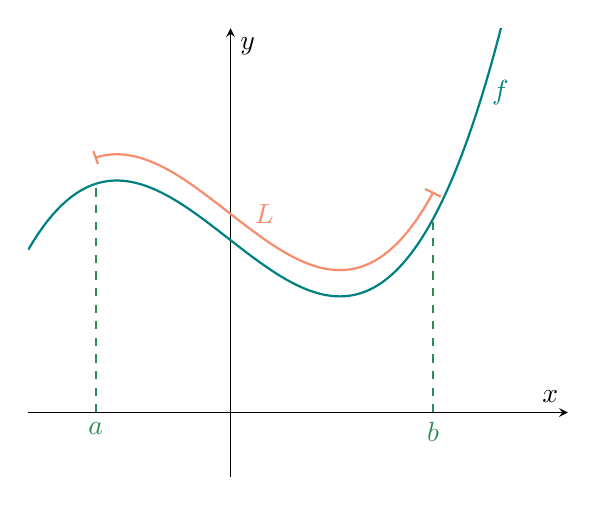
\begin{tikzpicture}
	\begin{axis}[
	axis lines = center, 
	xlabel = $x$, ylabel = $y$, 
	xmin = -3, xmax = 5, 
	ymin = -1, ymax = 6,
	ticks = none, 
	]
		\addplot[color = teal, thick, domain = -3:5, samples = 500] {0.1*x^(3) + 0.01*x^(2) - 0.82*x + 2.69};
		\addplot[color = Melon, thick, domain = -2:3, samples = 500] {0.1*x^(3) + 0.01*x^(2) - 0.82*x + 3.1};
		\draw[color = Melon, thick] (axis cs: {-0.34 * 0.1 - 2} , 0.1 + 3.57 + 0.41) --
		 (axis cs: {0.34 * 0.1 - 2}, -0.1 + 3.57 + 0.41);
		\draw[color = Melon, thick] (axis cs: {-1.94 * 0.06 + 3} , 0.06 + 3.02 + 0.41) --
		 (axis cs: {1.94 * 0.06 + 3}, -0.06 + 3.02 + 0.41);
		\node[color = teal] at (axis cs: 4,5) {$f$};
		\node[color = SeaGreen, anchor = north] at (axis cs: -2,0) {$a$};
		\node[color = SeaGreen, anchor = north] at (axis cs: 3,0) {$b$};
		\draw[color = SeaGreen, dashed, thick] (axis cs: -2,0) -- (axis cs: -2,3.57);
		\draw[color = SeaGreen, dashed, thick] (axis cs: 3,0) -- (axis cs: 3,3.02);
		\node[color = Melon, anchor = south] at (axis cs: 0.5,2.3+0.5) {$L$}; 
	\end{axis}
	\end{tikzpicture}
	\caption{Kurvelængden \textcolor{Melon}{$L$} på intervallet $[a,b]$.}
	\label{fig:kurve}
\end{figure}
Ønsker vi at bestemme kurvelængden for en differentiabel funktion, kan vi anvende følgende sætning. 
\begin{setn}[Kurvelængde]
	Kurvelængden for en differentiabel funktion $f$ på intervallet $[a,b]$ er givet ved
	\begin{align*}
		\int_a^b \sqrt{1 + (f'(x))^2} dx
	\end{align*}
\end{setn}
\begin{proof}
	Vi tager udgangspunkt i Figur \ref{fig:kurvebevis}. Vi lægger ud med at antage, at $f$ er differentiabel.
	\begin{figure}[H]
	\centering
	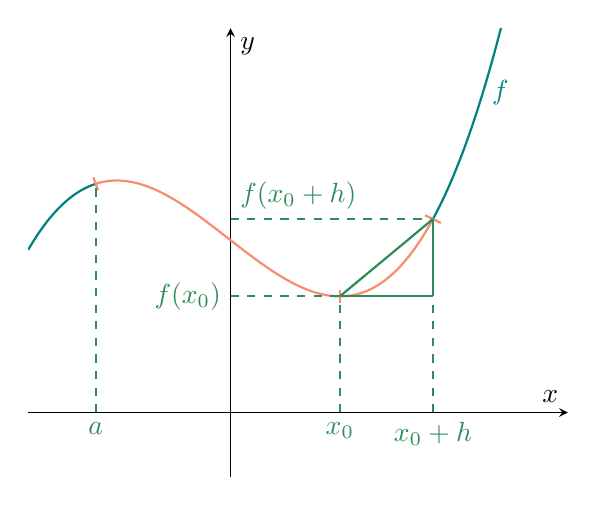
\begin{tikzpicture}
	\begin{axis}[
	axis lines = center, 
	xlabel = $x$, ylabel = $y$, 
	xmin = -3, xmax = 5, 
	ymin = -1, ymax = 6,
	ticks = none, 
	]
		\addplot[color = teal, thick, domain = -3:-2, samples = 500] {0.1*x^(3) + 0.01*x^(2) - 0.82*x + 2.69};
		\addplot[color = teal, thick, domain = 3:5, samples = 500] {0.1*x^(3) + 0.01*x^(2) - 0.82*x + 2.69};
		\addplot[color = Melon, thick, domain = -2:3, samples = 500] {0.1*x^(3) + 0.01*x^(2) - 0.82*x + 2.69};
		\draw[color = Melon, thick] (axis cs: {-0.34 * 0.1 - 2} , 0.1 + 3.57 ) --
		 (axis cs: {0.34 * 0.1 - 2}, -0.1 + 3.57  );
		\node[color = teal] at (axis cs: 4,5) {$f$};
		%Ticks and dashes
		\node[color = SeaGreen, anchor = north] at (axis cs: -2,0) {$a$};
		\node[color = SeaGreen, anchor = north] at (axis cs: 1.62,0) {$x_0$};
		\node[color = SeaGreen, anchor = north] at (axis cs: 3,0) {$x_0 + h$};
		\node[color = SeaGreen, anchor = east] at (axis cs: 0,1.813) {$f(x_0)$};
		\node[color = SeaGreen, anchor = south west] at (axis cs: 0,3.02) {$f(x_0 + h)$};
		\draw[color = SeaGreen, dashed, thick] (axis cs: -2,0) -- (axis cs: -2,3.57);
		\draw[color = SeaGreen, dashed, thick] (axis cs: 1.62,0) -- (axis cs: 1.62,1.813);
		\draw[color = SeaGreen, dashed, thick] (axis cs: 3,0) -- (axis cs: 3,3.02);
		\draw[color = SeaGreen, dashed, thick] (axis cs: 0,1.813) -- (axis cs: 1.62,1.813);
		\draw[color = SeaGreen, dashed, thick] (axis cs: 0,3.02) -- (axis cs: 3,3.02);
		%
		\draw[color = Melon, thick] (axis cs: 1.62 , 1.813 + 0.1) --
		 (axis cs: 1.62, 1.813 - 0.1);
		 \draw[color = Melon, thick] (axis cs: {-1.94 * 0.06 + 3} , 0.06 + 3.02 ) --
		 (axis cs: {1.94 * 0.06 + 3}, -0.06 + 3.02);
		%Triangle
		\draw[color = SeaGreen, thick] (axis cs: 1.62,1.813) -- (axis cs: 3,3.02);
		\draw[color = SeaGreen, thick] (axis cs: 1.62,1.813) -- (axis cs: 3,1.813);
		\draw[color = SeaGreen, thick] (axis cs: 3,1.813) -- (axis cs: 3,3.02);
	\end{axis}
	\end{tikzpicture}
	\caption{Approksimation af kurvelængde med ret linje.}
	\label{fig:kurvebevis}
	\end{figure}
	Vi antager, at vi har en kurvelængdefunktion $L_a(x)$, der giver os kurvelængden på intervallet $[a,x]$. Vi ønsker
	at betragte kurvelængden $L_a(x_0 + h)$ som set på Figur \ref{fig:kurvebevis}, og til dette skal vi bruge trekanten
	på figuren. Bredden af trekanten må være $h$ og højden af trekanten $f(x_0 + h) - f(x_0)$. Derfor giver 
	Pythagoras' sætning, at længden af hypotenusen i trekanten er
	\begin{align*}
		\sqrt{h^2 + \left(f(x_0 + h)- f(x_0)\right)^2}.
	\end{align*}
	Det må gælde, at den sande kurvelængde $L_a(x_0 + h)$ er approksimativt lig kurvelængden indtil $x_0$ lagt sammen 
	med længden af hypotenusen i trekanten. Derfor
	\begin{align*}
		L_a(x_0 + h) \approx L_a(x_0) + \sqrt{h^2 + \left(f(x_0 + h) - f(x_0)\right)^2}.
	\end{align*}
	Vi trækker $L_a(x_0)$ fra og dividerer med $h$.
	\begin{align*}
		&L_a(x_0 + h) \approx L_a(x_0) + \sqrt{h^2 + \left(f(x_0 + h) - f(x_0)\right)^2} \\
		\Leftrightarrow	\ &L_a(x_0 + h) - L_a(x_0) \approx  \sqrt{h^2 + \left(f(x_0 + h) - f(x_0)\right)^2} \\
		\Leftrightarrow	\ &\frac{L_a(x_0 + h) - L_a(x_0)}{h} \approx  
		 \frac{\sqrt{h^2 + \left(f(x_0 + h) - f(x_0)\right)^2}}{h}.
	\end{align*}
	Før vi lader $h \to 0$, så skriver vi lidt om på højresiden.
	\begin{align*}
		\frac{L_a(x_0 + h) - L_a(x_0)}{h} &\approx  \frac{\sqrt{h^2 + \left(f(x_0 + h) - f(x_0)\right)^2}}{h} \\
		&= \frac{\sqrt{h^2 + \left(f(x_0 + h) - f(x_0)\right)^2}}{\sqrt{h^2}} \\
		&= \sqrt{\frac{h^2 + \left(f(x_0 + h) - f(x_0)\right)^2}{h^2}} \\ 
		&= \sqrt{1 + \left(\frac{f(x_0 + h) - f(x_0)}{h}\right)^2}
	\end{align*}
	Vi kan nu se vores differenskvotient og vi lader derfor $h \to 0$. Når $h \to 0$, bliver vores approksimation en 
	lighed, og vi får
	\begin{align*}
		&\lim_{h \to 0}\frac{L_a(x_0 + h) - L_a(x_0)}{h} =
		 \lim_{h \to 0}\sqrt{1 + \left(\frac{f(x_0 + h) - f(x_0)}{h}\right)^2} \\
		 \Leftrightarrow \ &L_a'(x_0) = \sqrt{1+(f'(x_0))^2}.
	\end{align*}
	Derfor er $L_a$ en stamfunktion til $\sqrt{1+(f'(x))^2}$ og vi får
	\begin{align*}
		\int_a^b \sqrt{1+(f'(x))^2} dx = L_a(b) - L_a(a) = L_a(b),
	\end{align*}
	hvilket er netop kurvelængden fra $a$ til $b$. 
\end{proof}

\begin{exa}
	Vi ønsker at bestemme kurvelængden af funktionen $f$ givet ved
	\begin{align*}
		f(x) = x^2 + 4x - 5
	\end{align*}
	på intervallet $[2,9]$. Vi anvender typisk et CAS-værktøj til at bestemme kurvelængder, og vi bestemmer dem
	numerisk, da integraler der indeholder kvadratrødder kun sjældent kan løses eksakt. 
	Vi anvender integralværktøjet i paletten i Maple og får
	\begin{align*}
		\int_2^9 \sqrt{1 + (2x + 4)^2} dx = 105.25.
	\end{align*}
\end{exa}
\subsection*{Opgave 1 (Med Maple)}
Funktionen $g$ givet ved 
\begin{align*}
	g(x) = x^2 + 4x - 5
\end{align*}
roteres omkring $x$-aksen som set på Figur \ref{fig:omdrejningopg1}.
\begin{figure}[H]
	\centering
	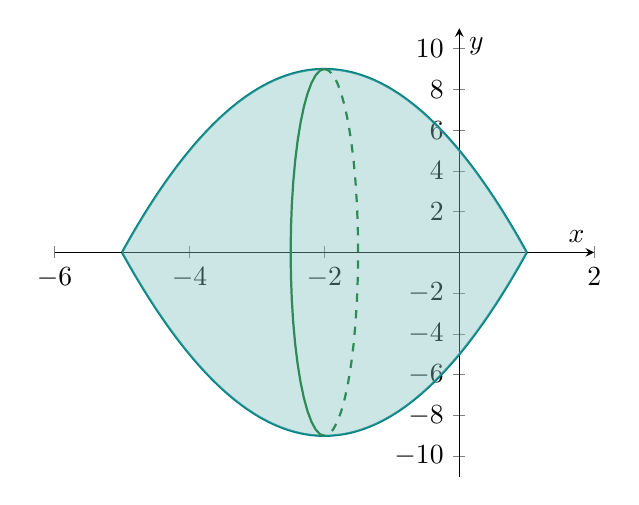
\begin{tikzpicture}
	\begin{axis}[
	axis lines = center, 
	xmin = -6, xmax = 2,
	ymin = -11, ymax = 11,
	xlabel = $x$, ylabel = $y$,
	xtick = {-8,-6,...,6,8}, ytick = {-12,-10,...,10,12},
	]
		\addplot[color = teal, thick, domain = -5:1, samples = 500] {x^2 + 4*x - 5};
		\addplot[color = teal, thick, domain = -5:1, samples = 500] {-x^2 - 4*x + 5};
		%Filling
		\fill[color = teal!50, opacity = 0.4] 
		plot[domain = -5:1, variable = \x] (axis cs: \x, {(\x)^2 + 4*\x - 5}) --
		plot[domain = 1:-5, variable = \x] (axis cs: \x, {-(\x)^2 - 4*\x + 5}) -- cycle;
		%Circles
		%circle
		\draw[color = SeaGreen, thick]
		plot[domain = 90:270, variable = \t] (axis cs: {0.5*cos(\t) - 2} , {9 * sin(\t)});
		\draw[color = SeaGreen, thick, dashed]
		plot[domain = 90:-90, variable = \t] (axis cs: {0.5*cos(\t) - 2} , {9 * sin(\t)}); 
	\end{axis}
	\end{tikzpicture}
	\caption{Omdrejningslegeme for funktion $g$.}
	\label{fig:omdrejningopg1}
\end{figure}

Bestem rumfanget af omdrejningslegemet.

\subsection*{Opgave 2 (Med Maple)}

Funktionerne $g$ og $h$ er givet ved henholdsvis
\begin{align*}
	g(x) = \frac{2}{5}x^3-2x^2+2x+4
\end{align*}
og
\begin{align*}
	h(x) = \frac{1}{2}(x-2)^2 + 1.
\end{align*}
Når de roteres om $x$-aksen, danner mellemrummet mellem deres omdrejningslegemer en skal til en krukke. 
\begin{figure}[H]
	\centering
	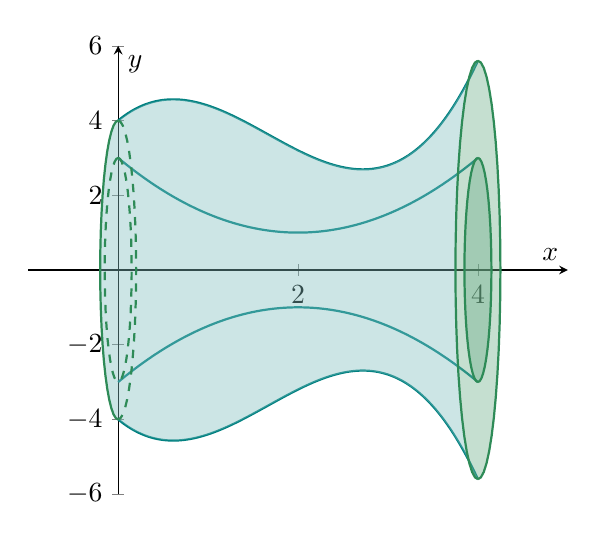
\begin{tikzpicture}
	\begin{axis}[
	axis lines = center, 
	xmin = -1, xmax = 5,
	ymin = -6, ymax = 6,
	xlabel = $x$, ylabel = $y$,
	xtick = {-8,-6,...,6,8}, ytick = {-12,-10,...,10,12},
	]
		\addplot[color = teal, thick, domain = -0:4, samples = 500] {0.4*x^3-2*x^2+2*x+4};
		\addplot[color = teal, thick, domain = -0:4, samples = 500] {-(0.4*x^3-2*x^2+2*x+4)};
		\addplot[color = teal, thick, domain = -0:4, samples = 500] {0.5*(x-2)^2+1};
		\addplot[color = teal, thick, domain = -0:4, samples = 500] {-0.5*(x-2)^2-1};
		%Filling
		\fill[color = teal!50, opacity = 0.4] 
		plot[domain = 0:4, variable = \x] (axis cs: \x, {0.4*\x^3-2*(\x)^2+2*\x+4}) --
		plot[domain = 90:270, variable = \t] (axis cs: {0.25*cos(\t) + 4} , {28/5 * sin(\t)}) -- 
		plot[domain = 4:0, variable = \x] (axis cs: \x, { -0.4*\x^3 + 2*(\x)^2 - 2*\x - 4}) -- 
		plot[domain = 270:90, variable = \t] (axis cs: {0.2*cos(\t) } , {4 * sin(\t)}) -- cycle;
		%Circle fill
		\fill[color = SeaGreen!70, opacity = 0.4] 
		plot[domain = 0:360, variable = \t] (axis cs: {0.25*cos(\t) + 4} , {28/5 * sin(\t)}) -- cycle;
		\fill[color = SeaGreen!70, opacity = 0.4] 
		plot[domain = 0:360, variable = \t] (axis cs: {0.15*cos(\t) + 4} , {3 * sin(\t)}) -- cycle;
		%Circles
		%left circles
		\draw[color = SeaGreen, thick]
		plot[domain = 90:270, variable = \t] (axis cs: {0.2*cos(\t) } , {4 * sin(\t)});
		\draw[color = SeaGreen, thick, dashed]
		plot[domain = 90:-90, variable = \t] (axis cs: {0.2*cos(\t)} , {4 * sin(\t)}); 
		\draw[color = SeaGreen, thick, dashed]
		plot[domain = 90:270, variable = \t] (axis cs: {0.15*cos(\t)} , {3 * sin(\t)});
		\draw[color = SeaGreen, thick, dashed]
		plot[domain = 90:-90, variable = \t] (axis cs: {0.15*cos(\t)} , {3 * sin(\t)}); 
		%right circles
		\draw[color = SeaGreen, thick]
		plot[domain = 90:270, variable = \t] (axis cs: {0.25*cos(\t) + 4} , {28/5 * sin(\t)});
		\draw[color = SeaGreen, thick]
		plot[domain = 90:-90, variable = \t] (axis cs: {0.25*cos(\t) + 4} , {28/5 * sin(\t)}); 
		\draw[color = SeaGreen, thick]
		plot[domain = 90:270, variable = \t] (axis cs: {0.15*cos(\t) + 4} , {3 * sin(\t)});
		\draw[color = SeaGreen, thick]
		plot[domain = 90:-90, variable = \t] (axis cs: {0.15*cos(\t) + 4} , {3 * sin(\t)}); 
	\end{axis}
	\end{tikzpicture}
	\caption{Omdrejningslegeme for funktionerne $g$ og $h$.}
	\label{fig:omdrejningopg2}
\end{figure}
Bestem rumfanget af denne krukke. 

\subsection*{Opgave 3 (med Maple)}
Omdrejningslegemerne på intervallet $[0,a$] for funktionerne $f$ og $g$ givet ved
\begin{align*}
	f(x) = 0.06x^3 - 0.61x^2 + 1.63x + 3
\end{align*}
og
\begin{align*}
	f(x) = 0.06x^3 - 0.61x^2 + 1.63x + 3.3
\end{align*}
danner til sammen en krukke
\begin{enumerate}[label=\roman*)]
	\item Tegn graferne for $f$ og $g$ i samme koordinatsystem.
	\item Bestem krukkens højde, så rumfanget af krukkens materiale er 3.
\end{enumerate}

\subsection*{Opgave 4 (med Maple)}
\begin{enumerate}[label=\roman*)]
	\item Bestem kurvelængden af $f(x) = x^3$ på intervallet $[-2,10]$.
	\item Bestem kurvelængden af $f(x) = \sqrt{x}$ på intervallet $[0,16]$.
	\item Bestem kurvelængden af $f(x) = e^x$ på intervallet $[0,1]$.
	\item Bestem kurvelængden af $f(x) = \ln(x)$ på intervallet $[e,e^2]$.
\end{enumerate}

\subsection*{Opgave 5}
\begin{enumerate}[label=\roman*)]
	\item Vis, at rumfanget af en kegle med radius $r$ og højde $h$ er givet ved
	\begin{align*}
		\frac{\pi}{3}hr^2
	\end{align*}
	ved at bruge formlen for rumfanget af omdrejningslegemer
\end{enumerate}
\subsection*{Opgave 6}
En cirkels ligning er givet ved 
\begin{align*}
	x^2 + y^2 = r^2,
\end{align*}
hvor $r$ er cirklens radius og cirklen har centrum i origo. 
\begin{enumerate}[label=\roman*)]
	\item Isolér $y$ i cirklens ligning. 
	\item Brug formlen for rumfanget af omdrejningslegemer til at vise, at rumfanget af en kugle er
	\begin{align*}
		\frac{4\pi}{3}r^3
	\end{align*}
\end{enumerate}